\section{Ergebnis} % (fold)
\label{sec:ergebnis}
	Bereits zu Beginn des Projekts war es wichtig es messbar zu machen. Dafür wurde eine Testumgebung aufgebaut, mit deren Hilfe die Seite nach ihrer Geschwindigkeit getestet werden kann. Ganz entscheidend war dabei die Webpagetest API in Verbindung mit Google Spreadsheets. Damit lassen sich regelmäßig automatisierte Tests durchführen und die Daten werden nach erfolgreichem Test automatisch in einer Spreadsheet Tabelle gespeichert. Die über den Zeitraum der Arbeit hinweig gesammelten Daten sind hier finden: \url{http://tinyurl.com/l5usz79}. Diese Daten wurden anschließend mittels \url{http://Chartjs.org} in Diagrammen aufbereitet und sind unter: \url{http://bithugger.github.io/bachelorthesis/} zu finden.

	\subsubsection{Wie wurde getestet?} % (fold)
	\label{ssub:wie_wurde_getestet}
		Damit mittels Google Spreadsheets die Webpagetest API verwendet werden kann, ist es nötig einen sogenannten API-Key anzufordern. Ein solcher Key ist kostenlos unter der Adresse: \url{http://www.webpagetest.org/getkey.php} zu erhalten und bietet die Möglichkeit täglich 200 Seitenaufrufe zu tätigen. Als Seitenaufruf zählt sowohl die "`first view"' als auch "`repeat view"'. Die Tests sind 30 Tage abrufbar und gespeichert.\\

		Für das Testen der Seite kann aus einer Vielzahl an Teststandorten gewählt werden. Damit lässt sich nachvollziehen wie beispielsweise die Ladezeiten aus der USA oder Asien sind. Je nach Zielgruppe sollten Tests von verschiedenen Standorten in betracht gezogen werden.\footnote{Eine volle Liste der zur Verfügung stehenden Teststandorte ist im Anhang unter Punkt: \ref{sub:webpagetest_teststandorte} zu finden.} Für dieses Projekt wurden ausschließlich Teststandorte aus der USA und Europa gewählt.\\

		- Testparameter (first view, \#runs)
		- Aufgezeichnete Daten
		- Probleme?

	% subsubsection wie_wurde_getestet (end)

		1089 Testläufe über Webpagtest: Zeitraum: 1 Monat

		\begin{figure}[htbp]
			\begin{center}
				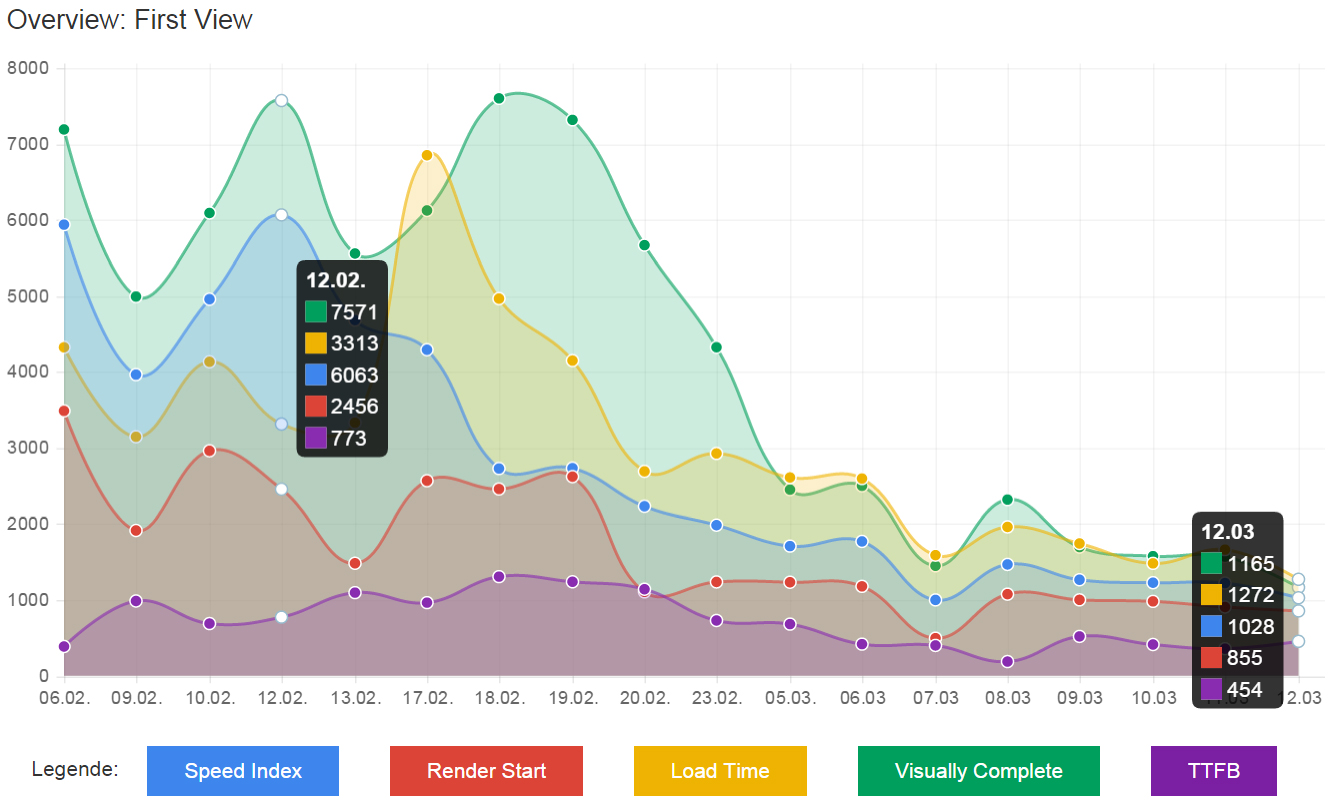
\includegraphics[width=\textwidth]{data_all.jpg}
				\caption{...}
				\label{fig:data_all}
			\end{center}
		\end{figure}

	% section ergebnis (end)
